%!TEX root = ../main.tex
\subsection{Threshold correlations}
\begin{figure}[H]
  \caption{Threshold correlations on weekly data}
  \label{diag:thresholdweekly}
  \centering
  \begin{minipage}{\textwidth}
  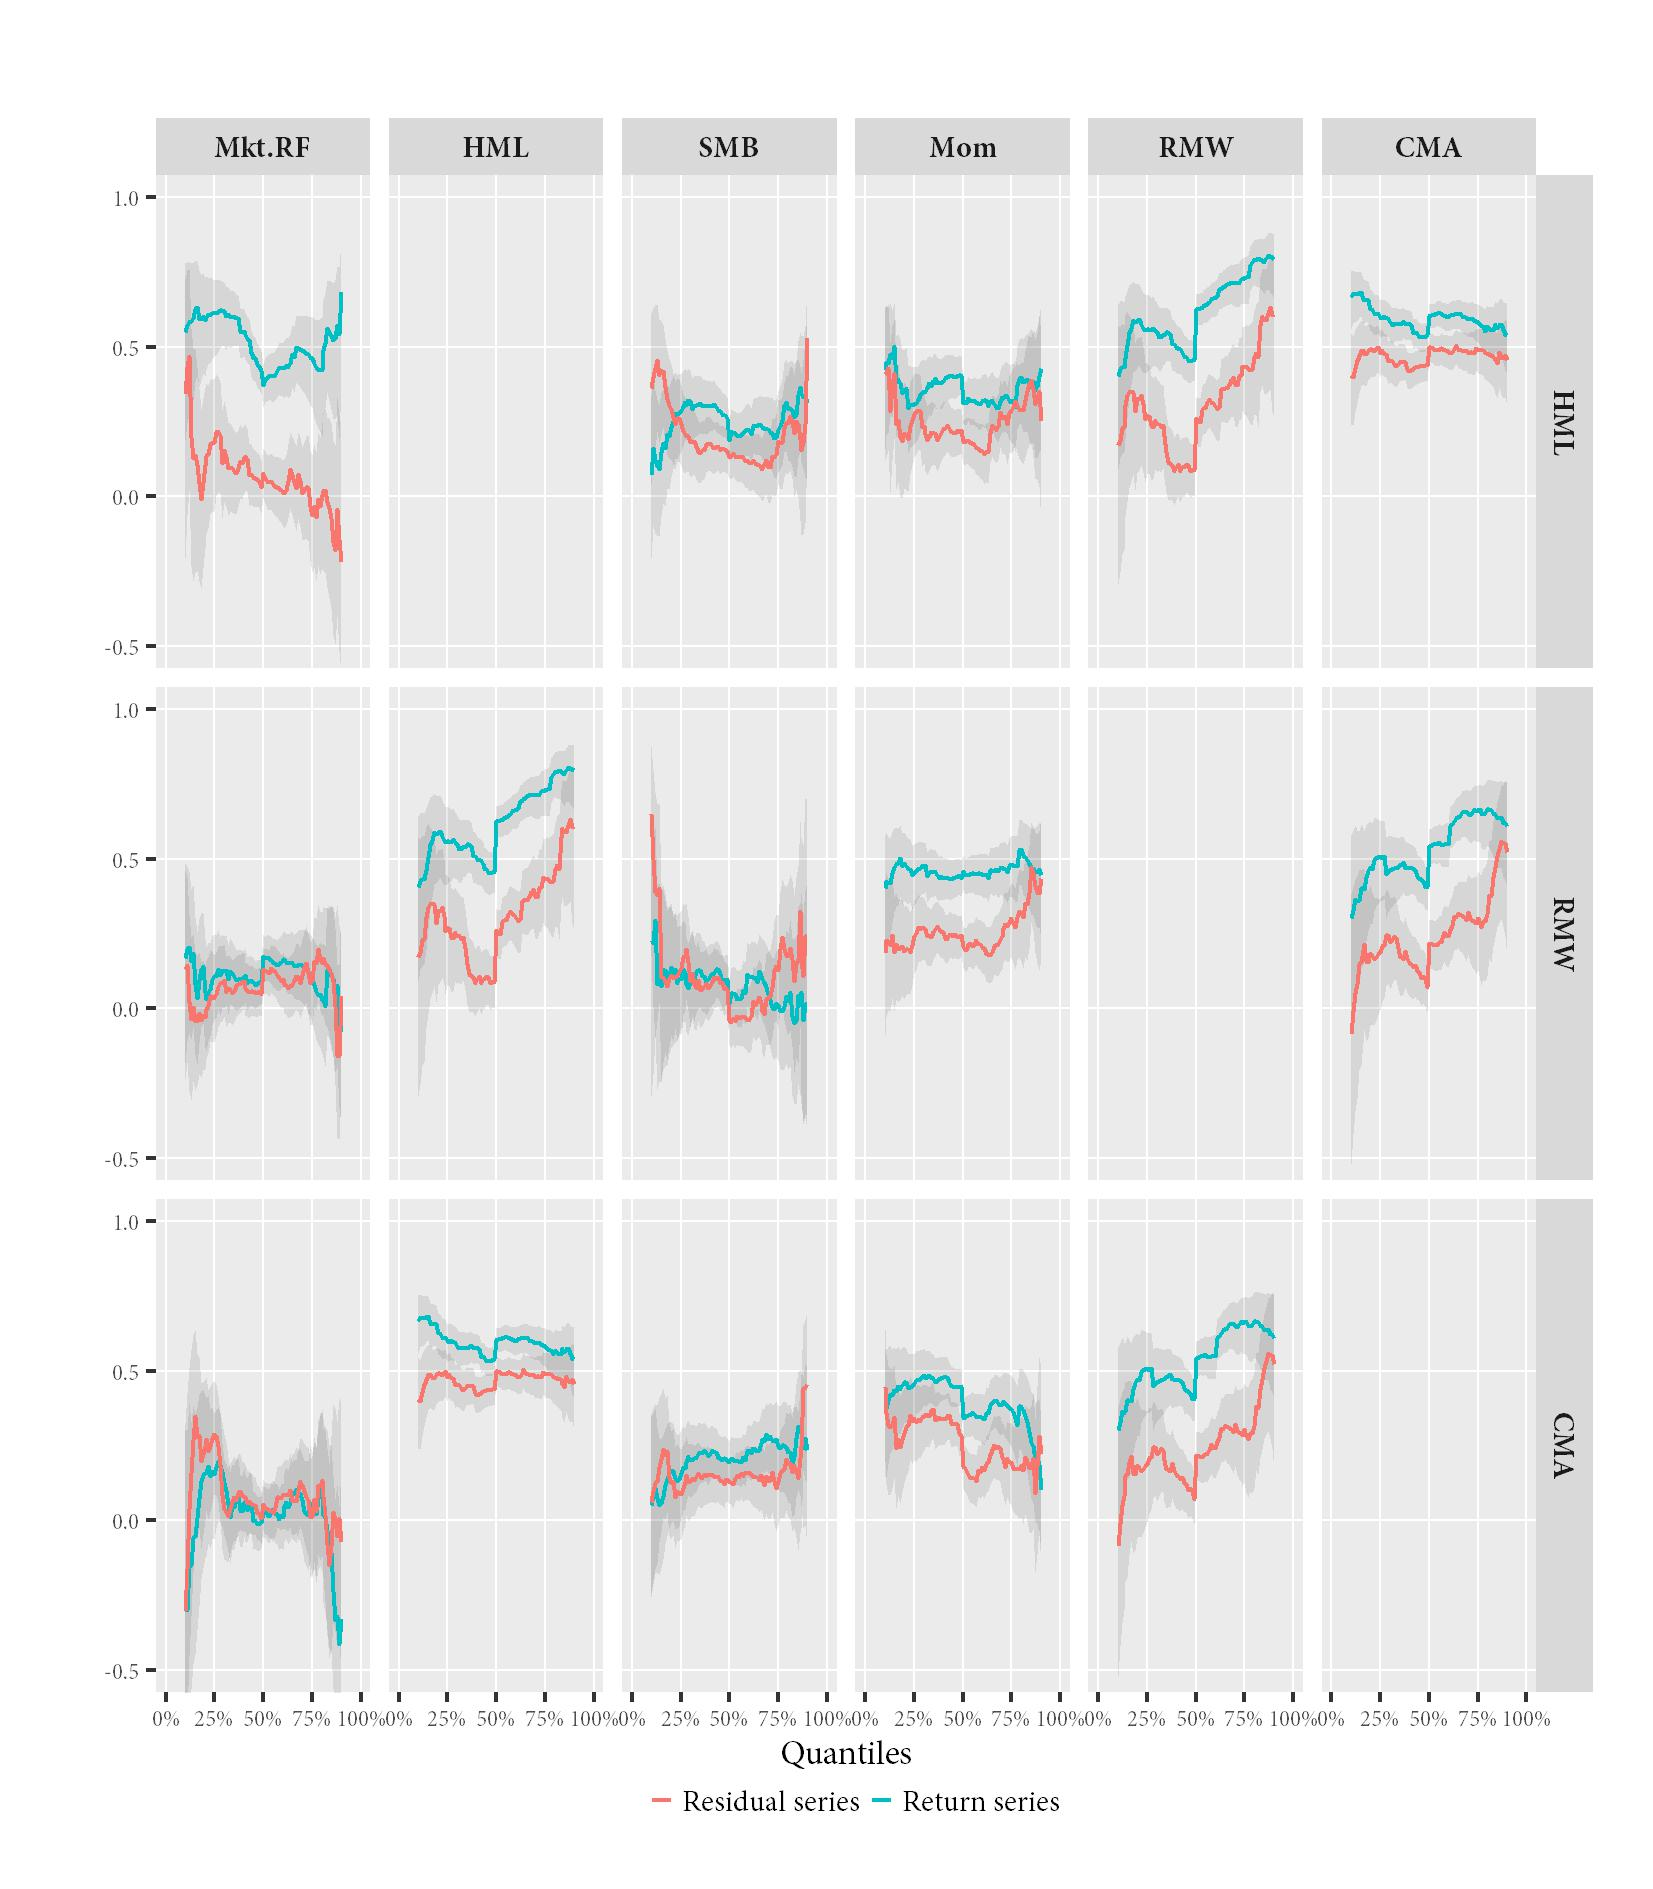
\includegraphics[scale=1]{graphics/thresholdweekly.jpeg}  
  \footnotesize
  \textit{Note:} Lorem ipsum dolor sit amet, consectetur adipiscing elit, sed do eiusmod tempor incididunt ut labore et dolore magna aliqua. Ut enim ad minim veniam, quis nostrud exercitation ullamco laboris nisi ut aliquip ex ea commodo consequat. Duis aute irure dolor in reprehenderit in voluptate velit esse cillum dolore eu fugiat nulla pariatur. Excepteur sint occaecat cupidatat non proident, sunt in culpa qui officia deserunt mollit anim id est laborum.
  \end{minipage}
\end{figure}

\begin{itemize}
  \item There is a marked difference between the threshold correlations before and after applying a GARCH filter. We conclude that a large part of what intially seems as multivariate asymmetry is in fact due to simultaneous ARMA-GARCH effects on the marginal level (reference to market hml graph for example)
  \item Still, there is a lot of tail dependence and asymmetry left. [A Gaussian model with linear correlations approaches zero correlation when the quantile goes to zero and one respectively.] Refernce tail dependency to any graph, reference asymmetry to mkt hml, rmw hml, mom hml, mom cma. 
  \item Market HML is not what you want! others are nicer. supports hypothesis indicative  
\end{itemize}
\subsection{Copula results}
% TABLES NEED TO BE MODIFIED IN THE FOLLOWING WAYS
% 1) Change {tabular} to {tabularx}{\textwidth} and make leftmost column an X column
%     and change top and bottom \hline to \toprule \bottomrule
%
% paste the following at start but before & \multicolumn
%
% \begin{tabularx}{\textwidth}{@{\extracolsep{5pt}} X D{.}{.}{-3} D{.}{.}{-3} D{.}{.}{-3} } 
% \\[-1.8ex] \midrule
% \\[-1.8ex] 
%
% paste the following at end after R2 row but before Note row
% \bottomrule \\[-1.8ex] 
%
% 2) Change the variable names to greeks
% 3) Change specification names if needed
% 4) Change R2 to LLH and add similar lines for Ljung-Box and ARCH-LM
% 5) Add label and caption
% 6) Paste this to get table heading description
%
% \begin{tabularx}{\textwidth}{X}
% \\[-1.8ex]\toprule
%\\[-1.8ex] 
% text goes here
% \end{tabularx}
%
% 6) Copy the whole table, only change caption, label, factor/spec labels and (1)-(3) to (4)-(6)
% Table created by stargazer v.5.2 by Marek Hlavac, Harvard University. E-mail: hlavac at fas.harvard.edu
% Date and time: ons, okt 12, 2016 - 12:37:02
% Requires LaTeX packages: dcolumn 
\begin{table}[!htbp] \centering 
  \caption{Copula results: Constant specifications} 
  \label{tab:copula1} 
\begin{tabularx}{\textwidth}{X}
  \\[-1.8ex]\toprule
  \\[-1.8ex] 
  \footnotesize Lorem ipsum dolor sit amet, consectetur adipiscing elit, sed do eiusmod tempor incididunt ut labore et dolore magna aliqua. Ut enim ad minim veniam, quis nostrud exercitation ullamco laboris nisi ut aliquip ex ea commodo consequat. Duis aute irure dolor in reprehenderit in voluptate velit esse cillum dolore eu fugiat nulla pariatur. Excepteur sint occaecat cupidatat non proident, sunt in culpa qui officia deserunt mollit anim id est laborum.
\end{tabularx}
\begin{tabularx}{\textwidth}{@{\extracolsep{5pt}} X D{.}{.}{-3} D{.}{.}{-3} D{.}{.}{-3} } 
  \\[-1.8ex]\midrule
  \\[-1.8ex] 
   & \multicolumn{3}{c}{Constant copula models} \\ 
  \cline{2-4} 
  \\[-1.8ex] & \multicolumn{1}{c}{(1)} & \multicolumn{1}{c}{(2)} & \multicolumn{1}{c}{(3)}\\ 
  \\[-1.8ex] & \multicolumn{1}{c}{Gaussian} & \multicolumn{1}{c}{Student-\textit{t}} & \multicolumn{1}{c}{Skewed Student-\textit{t}}\\ 
  \hline \\[-1.8ex] 
 $\nu$ &  & 6.508 & 6.566 \\ 
  &  & () & () \\ 
  & & & \\ 
 $\gamma_{Mkt.RF}$ &  &  & -0.019 \\ 
  &  &  & () \\ 
  & & & \\ 
 $\gamma_{HML}$ &  &  & 0.090 \\ 
  &  &  & () \\ 
  & & & \\ 
 $\gamma_{SMB}$ &  &  & -0.083 \\ 
  &  &  & () \\ 
  & & & \\ 
 $\gamma_{Mom}$ &  &  & -0.172 \\ 
  &  &  & () \\ 
  & & & \\ 
 $\gamma_{RMW}$ &  &  & 0.011 \\ 
  &  &  & () \\ 
  & & & \\ 
 $\gamma_{CMA}$ &  &  & 0.079 \\ 
  &  &  & () \\ 
  & & & \\ 
 $\alpha$ & 0 & 0 & 0 \\ 
  &  &  &  \\ 
  & & & \\ 
 $\beta$ & 0 & 0 & 0 \\ 
  &  &  &  \\ 
  & & & \\ 
\hline \\[-1.8ex] 
Observations & \multicolumn{1}{c}{2,479} & \multicolumn{1}{c}{2,479} & \multicolumn{1}{c}{2,479} \\ 
LLH & \multicolumn{1}{c}{1,096} & \multicolumn{1}{c}{1,463} & \multicolumn{1}{c}{1,475} \\ 
\bottomrule \\[-1.8ex] 
\textit{Note:}  & \multicolumn{3}{c}{$^{*}$p$<$0.1; $^{**}$p$<$0.05; $^{***}$p$<$0.01} \\ 
\end{tabularx} 
\end{table} 
% Table created by stargazer v.5.2 by Marek Hlavac, Harvard University. E-mail: hlavac at fas.harvard.edu
% Date and time: ons, okt 12, 2016 - 12:37:02
% Requires LaTeX packages: dcolumn 
\begin{table}[!htbp] \centering 
  \caption{Copula results: \textit{c}DCC specifications} 
  \label{tab:copula2} 
\begin{tabularx}{\textwidth}{X}
\\[-1.8ex]\toprule
\\[-1.8ex] 
\footnotesize Lorem ipsum dolor sit amet, consectetur adipiscing elit, sed do eiusmod tempor incididunt ut labore et dolore magna aliqua. Ut enim ad minim veniam, quis nostrud exercitation ullamco laboris nisi ut aliquip ex ea commodo consequat. Duis aute irure dolor in reprehenderit in voluptate velit esse cillum dolore eu fugiat nulla pariatur. Excepteur sint occaecat cupidatat non proident, sunt in culpa qui officia deserunt mollit anim id est laborum.
\end{tabularx}
\begin{tabularx}{\textwidth}{@{\extracolsep{5pt}} X D{.}{.}{-3} D{.}{.}{-3} D{.}{.}{-3} } 
\\[-1.8ex]\midrule
\\[-1.8ex] 
 & \multicolumn{3}{c}{Dynamic copula models} \\ 
\cline{2-4} 
\\[-1.8ex] & \multicolumn{1}{c}{(4)} & \multicolumn{1}{c}{(5)} & \multicolumn{1}{c}{(6)}\\ 
\\[-1.8ex] & \multicolumn{1}{c}{Gaussian} & \multicolumn{1}{c}{Student-\textit{t}} & \multicolumn{1}{c}{Skewed Student-\textit{t}}\\ 
\hline \\[-1.8ex] 
 $\nu$ &  & 11.831 & 11.803 \\ 
  &  & () & () \\ 
  & & & \\ 
 $\gamma_{Mkt.RF}$ &  &  & -0.055 \\ 
  &  &  & () \\ 
  & & & \\ 
 $\gamma_{HML}$ &  &  & 0.071 \\ 
  &  &  & () \\ 
  & & & \\ 
 $\gamma_{SMB}$ &  &  & -0.170 \\ 
  &  &  & () \\ 
  & & & \\ 
 $\gamma_{Mom}$ &  &  & -0.125 \\ 
  &  &  & () \\ 
  & & & \\ 
 $\gamma_{RMW}$ &  &  & 0.095 \\ 
  &  &  & () \\ 
  & & & \\ 
 $\gamma_{CMA}$ &  &  & 0.022 \\ 
  &  &  & () \\ 
  & & & \\ 
 $\alpha$ & 0.066 & 0.068 & 0.068 \\ 
  & () & () & () \\ 
  & & & \\ 
 $\beta$ & 0.915 & 0.913 & 0.913 \\ 
  & () & () & () \\ 
  & & & \\ 
\hline \\[-1.8ex] 
Observations & \multicolumn{1}{c}{2,766} & \multicolumn{1}{c}{2,766} & \multicolumn{1}{c}{2,766} \\ 
LLH & \multicolumn{1}{c}{2,791} & \multicolumn{1}{c}{2,975} & \multicolumn{1}{c}{2,984} \\ 
\bottomrule \\[-1.8ex] 
\textit{Note:}  & \multicolumn{3}{c}{$^{*}$p$<$0.1; $^{**}$p$<$0.05; $^{***}$p$<$0.01} \\ 
\end{tabularx} 
\end{table} 
\begin{itemize}
  \item Large step up in LLH from constant to dynamic copula. Consistent with fact that correlations vary over time. Reference to graph
  \item Asymmetry parameters generally significantly estimated, but the change in LLH is not as great as for the change from the normal specification
  \item Comment on variance non-persistence
  \item Vuong test conclusion
\end{itemize}
\subsection{Conditional diversification benefit}